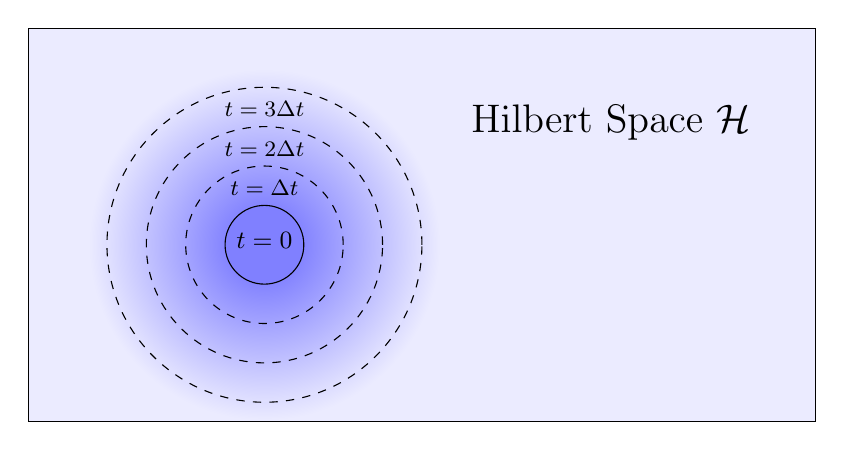
\begin{tikzpicture}[inner sep=1mm]

\node[rectangle,draw=black,fill=blue!8,minimum height=5cm,minimum width=10cm] (H) at (0,0) {};


\shade[inner color=blue!60,outer color=blue!8] (-2,-0.25) circle [radius=2.22cm];
\shade[inner color=blue!60,outer color=blue!12] (-2,-0.25) circle [radius=2cm];

\draw[radius=1.0,draw=black,dashed] (-2,-0.25) circle;
\draw[radius=1.5,draw=black,dashed] (-2,-0.25) circle;
\draw[radius=2.0,draw=black,dashed] (-2,-0.25) circle;

\filldraw[radius=0.5,draw=black,fill=blue!50] (-2,-0.25) circle;

\node (H1) at (2.4,1.3) {\Large Hilbert Space $\mathcal{H}$};
\node (t0) at (-2,-0.2) {\small $t = 0$};
\node (t1) at (-2,0.47) {\footnotesize $t = \Delta t$};
\node (t2) at (-2,0.97) {\footnotesize $t = 2 \Delta t$};
\node (t3) at (-2,1.47) {\footnotesize $t = 3 \Delta t$};

\end{tikzpicture}